\documentclass[a4paper,12pt]{report}

% -------------------------------
% PACKAGES
% -------------------------------
\usepackage[utf8]{inputenc}
\usepackage[english]{babel}
\usepackage{graphicx}
\usepackage{fancyhdr}
\usepackage{geometry}
\usepackage{titlesec}
\usepackage{microtype}
\usepackage{xcolor}
\usepackage{ragged2e}
\usepackage{setspace}
\usepackage{parskip}
\usepackage{listings}
\usepackage{amsmath}
\usepackage{amsfonts}
\usepackage{amssymb}
\usepackage{float}
\usepackage{caption}
\usepackage{subcaption}
\usepackage{algorithm}
\usepackage{algorithmic}
\usepackage{tabularx}
\usepackage{longtable}
\usepackage{multirow}
\usepackage{booktabs}
\usepackage{hyperref}
\usepackage{url}
\usepackage{verbatim}
\usepackage{fancyvrb}
\usepackage{tcolorbox}
\usepackage{enumitem}

% -------------------------------
% PAGE SETUP
% -------------------------------
\geometry{top=0.6in, bottom=1in, left=1in, right=1in, headheight=15pt}
\setstretch{1.5}
\flushbottom

% -------------------------------
% CODE LISTING SETUP
% -------------------------------
\definecolor{codegreen}{rgb}{0,0.6,0}
\definecolor{codegray}{rgb}{0.5,0.5,0.5}
\definecolor{codepurple}{rgb}{0.58,0,0.82}
\definecolor{backcolour}{rgb}{0.95,0.95,0.92}

\lstset{
    basicstyle=\ttfamily\footnotesize,
    keywordstyle=\color{blue}\bfseries,
    commentstyle=\color{codegreen},
    stringstyle=\color{codepurple},
    numbers=left,
    numberstyle=\tiny\color{codegray},
    stepnumber=1,
    numbersep=8pt,
    showstringspaces=false,
    breaklines=true,
    frame=single,
    backgroundcolor=\color{gray!10},
    captionpos=b,
    aboveskip=6pt,
    belowskip=6pt,
    language=Python
}

% Hyperref setup
\hypersetup{
    colorlinks=true,
    linkcolor=blue,
    filecolor=magenta,
    urlcolor=cyan,
    pdftitle={Multi-Modal Human Pose and Gesture Estimation System},
    pdfsubject={Multimedia Analysis Project},
    pdfkeywords={Pose Estimation, Gesture Recognition, MediaPipe, Sign Language, Computer Vision},
    pdfpagelabels=true
}

% tcolorbox default style
\tcbset{
  colback=gray!5,
  colframe=black!60,
  boxrule=0.4pt,
  arc=2mm,
  boxsep=4pt,
}

% -------------------------------
% CHAPTER FORMAT FIX
% -------------------------------
\titleformat{\chapter}[hang]
  {\normalfont\bfseries\Large}
  {\thechapter.}{1em}{}
\titleformat{name=\chapter,numberless}[hang]
  {\normalfont\bfseries\Large}
  {}{0pt}{}
\titlespacing*{\chapter}{0pt}{-15pt}{10pt}

% -------------------------------
% HEADER & FOOTER STYLES
% -------------------------------
\fancypagestyle{firstpage}{
  \fancyhf{}
  \renewcommand{\headrulewidth}{0pt}
  \renewcommand{\footrulewidth}{0pt}
}

\fancypagestyle{contentpages}{
  \fancyhf{}
  \renewcommand{\headrulewidth}{0.4pt}
  \renewcommand{\footrulewidth}{0.4pt}
  \fancyhead[L]{\leftmark}
  \fancyfoot[C]{\thepage}
}

% ================================================================
% DOCUMENT START
% ================================================================
\begin{document}

% -------------------------------
% Title Page
% -------------------------------
\begin{titlepage}
  \thispagestyle{firstpage}
  \begin{center}

    % University Logo
    \begin{center}
      
\includegraphics[width=0.3\textwidth]{../IIITDM Kancheepuram_logo.png}\\[0.5cm]
    \end{center}

    {\LARGE \textbf{Indian Institute of Information Technology, Design and Manufacturing, Kancheepuram}}\\[0.5cm]
    {\large (Multimedia Analysis -- Project Report)}\\[3cm]

    \rule{\linewidth}{0.5pt}\\[0.4cm]
    {\Huge \textbf{Multi-Modal Human Pose \&}}\\[0.2cm]
    {\Huge \textbf{Gesture Estimation System}}\\[0.3cm]
    {\Large \textbf{Real-Time Analysis with Web Dashboard, Sign Language Recognition \& Gesture-Controlled Game}}\\[0.3cm]
    \rule{\linewidth}{0.5pt}\\[2cm]

    % Members
    \begin{minipage}{0.9\textwidth}
      \centering
      \begin{tabular}{l}
        \textbf{NAME} \\
        Roll Number \\
      \end{tabular}
    \end{minipage}

    \vfill
    {\large \today}

  \end{center}
\end{titlepage}

% -------------------------------
% Declaration
% -------------------------------
\chapter*{Declaration}
\thispagestyle{contentpages}
I hereby declare that this project report titled \textbf{``Multi-Modal Human Pose \& Gesture Estimation System''} is a bonafide record of work carried out by me as part of the course \textbf{Multimedia Analysis} at \textbf{IIITDM Kancheepuram}.
This report has not been submitted elsewhere for the award of any other degree or diploma.

\vspace{2cm}
\begingroup
\let\clearpage\relax

% -------------------------------
% Acknowledgment
% -------------------------------
\chapter*{Acknowledgment}
\thispagestyle{contentpages}
I would like to express my sincere gratitude to the course instructor for continuous support and encouragement throughout the course of this project.

I am also thankful to the \textbf{Department of Computer Science and Engineering, IIITDM Kancheepuram}, for providing the opportunity and facilities to undertake this project.

Special thanks to the open-source communities behind MediaPipe, OpenCV, and Flask for providing the foundational tools that made this system possible.

\vspace{1cm}
\begin{flushright}
\textbf{NAME}\\
Roll Number
\end{flushright}

\endgroup
\newpage

% -------------------------------
% Abstract
% -------------------------------
\chapter*{Abstract}
\thispagestyle{contentpages}
\addcontentsline{toc}{chapter}{Abstract}
\justifying
\noindent
This report presents a comprehensive \textbf{multi-modal real-time human analysis system} that simultaneously processes body pose, hand gestures, facial expressions, sign language recognition, and gesture-controlled interaction from a single webcam feed. The system employs Google's \textbf{MediaPipe} framework -- specifically BlazePose, Hand Tracking, and FaceMesh models -- to extract skeletal, hand, and facial landmarks, which are then analyzed through a pipeline of custom modules.

\par
The analysis pipeline computes \textbf{9 joint angles} with EMA smoothing, classifies \textbf{12+ hand gestures}, detects facial expressions via \textbf{Eye Aspect Ratio (EAR)} and \textbf{Mouth Aspect Ratio (MAR)}, counts exercise repetitions using angle-based state machines, analyzes bilateral pose symmetry, and recognizes \textbf{20 ASL alphabet letters} through geometric hand landmark classification.

\par
A \textbf{Flask-based web dashboard} provides an interactive browser interface with live MJPEG video streaming, analytics panels, a sign language translator, and a gesture-controlled dodging game. The system comprises \textbf{25+ source files}, supports both standalone OpenCV and web-based modes, and delivers real-time performance at 15--25 FPS on standard hardware.

\par
\textbf{Keywords:} Pose Estimation, MediaPipe, Gesture Recognition, Sign Language, EAR, MAR, Flask, Computer Vision, Real-Time Analysis, Exercise Tracking.

% Lists
\makeatletter
\let\l@table\l@figure
\renewcommand\listoffigures{%
    \section*{\listfigurename}%
    \@mkboth{\MakeUppercase\listfigurename}{\MakeUppercase\listfigurename}%
    \@starttoc{lof}%
}
\renewcommand\listoftables{%
    \section*{\listtablename}%
    \@mkboth{\MakeUppercase\listtablename}{\MakeUppercase\listtablename}%
    \@starttoc{lot}%
}
\makeatother

\clearpage
\pagenumbering{roman}
\setstretch{1.3}

\renewcommand{\contentsname}{Table of Contents}
\tableofcontents
\clearpage
\listoffigures
\clearpage
\listoftables

\clearpage
\pagenumbering{arabic}

% ================================================================
% Chapter 1: Introduction
% ================================================================
\chapter{Introduction}
\thispagestyle{contentpages}
\justifying

\section{Project Overview}
The \textbf{Multi-Modal Human Pose \& Gesture Estimation System} is an advanced real-time computer vision application that integrates multiple analysis engines to provide comprehensive human body understanding from a single webcam feed. Unlike traditional single-purpose pose estimators, this system simultaneously performs body pose estimation, hand gesture recognition, facial expression detection, activity classification, exercise tracking, symmetry analysis, sign language recognition, and gesture-controlled gaming.

The project is built on Google's MediaPipe framework and extends its capabilities through a modular pipeline of custom analysis engines, each implementing domain-specific algorithms and heuristics.

\section{Problem Statement}
Human pose estimation and gesture recognition are fundamental problems in computer vision with applications in:
\begin{itemize}
    \item \textbf{Healthcare:} Physical therapy monitoring, ergonomic assessment
    \item \textbf{Accessibility:} Sign language translation for the hearing impaired
    \item \textbf{Fitness:} Automated exercise form checking and repetition counting
    \item \textbf{Entertainment:} Gesture-controlled gaming and interactive experiences
    \item \textbf{HCI:} Natural human-computer interaction without controllers
\end{itemize}

Traditional approaches require specialized hardware (depth cameras, motion capture suits) or separate systems for each modality. This project addresses the challenge of integrating all these capabilities into a single, real-time, webcam-based system.

\section{Objectives}
The primary objectives of this project are:
\begin{enumerate}
    \item \textbf{Multi-Joint Kinematic Analysis:} Compute 9 joint angles with real-time smoothing
    \item \textbf{Gesture Vocabulary:} Classify 12+ hand gestures from landmark geometry
    \item \textbf{Expression Detection:} Detect blinks, yawns, talking, and head tilt using EAR/MAR
    \item \textbf{Activity Classification:} Identify 7 body postures with temporal debouncing
    \item \textbf{Exercise Counting:} Track repetitions for 5 exercises using state machines
    \item \textbf{Symmetry Analysis:} Compute bilateral joint symmetry scores
    \item \textbf{Sign Language:} Recognize 20 ASL alphabet letters geometrically
    \item \textbf{Gesture Game:} Create body-controlled interactive game
    \item \textbf{Web Dashboard:} Build browser-based interface with live analytics
    \item \textbf{Visualization:} Implement motion trails and real-time scrolling graphs
\end{enumerate}

\section{System Features at a Glance}
\begin{table}[H]
\centering
\begin{tabular}{|l|c|}
\hline
\textbf{Feature} & \textbf{Value} \\
\hline
Total Source Files & 25+ \\
Core Analysis Engines & 7 \\
Utility Modules & 6 \\
Web Dashboard Pages & 4 \\
Joint Angles Tracked & 9 \\
Gesture Vocabulary & 12+ \\
Activity Classifications & 7 \\
ASL Letters Supported & 20 \\
Exercise Types & 5 \\
Symmetry Joint Pairs & 4 \\
Keyboard Shortcuts (Standalone) & 11 \\
Recording Modes & 3 (CSV, Video, Snapshot) \\
Real-Time Graphs & 4 \\
Face Landmarks & 468 \\
\hline
\end{tabular}
\caption{System Feature Summary}
\label{tab:features}
\end{table}

% System Flow Diagram
\begin{figure}[H]
    \centering
    \begin{tcolorbox}[colback=blue!5, colframe=blue!40, width=0.95\textwidth, height=6cm]
        \centering
        \vfill
        \textbf{ANALYSIS PIPELINE FLOW}\\[0.6cm]
        \texttt{Webcam} $\rightarrow$ \texttt{Frame Capture} $\rightarrow$ \texttt{MediaPipe Models} $\rightarrow$ \texttt{Custom Analysis Engines} $\rightarrow$ \texttt{HUD / Web Dashboard}\\[0.4cm]
        \small
        \textit{Pose (33 lm) | Hands (21 lm) | Face (468 lm)} $\rightarrow$ \textit{Angles, Gestures, EAR/MAR, Activity, Exercise, Symmetry, Sign Language}
        \vfill
    \end{tcolorbox}
    \caption{Overview of the Real-Time Analysis Pipeline Flow}
    \label{fig:pipeline_flow}
\end{figure}

\newpage

% ================================================================
% Chapter 2: Literature Review
% ================================================================
\chapter{Literature Review and Background}
\thispagestyle{contentpages}
\justifying

\textbf{Human pose estimation} has evolved from classical approaches using Histogram of Oriented Gradients (HOG) and deformable part models to modern deep learning architectures. Recent advances in lightweight neural networks have made real-time inference possible on consumer hardware.

\section{MediaPipe Framework}
Google's MediaPipe \cite{mediapipe2019} provides a modular framework for building perception pipelines. It offers pre-trained models for face detection, hand tracking, and body pose estimation that run efficiently on CPUs and mobile GPUs.

\section{BlazePose}
BlazePose \cite{blazepose2020} detects 33 body landmarks in real-time using a lightweight CNN architecture. It achieves comparable accuracy to heavier models while maintaining interactive frame rates, making it ideal for real-time applications.

\section{Hand Tracking}
MediaPipe Hands \cite{handtracking2020} provides 21-landmark hand tracking using a two-stage pipeline: palm detection followed by precise landmark regression. This enables detailed finger state analysis and gesture classification.

\section{Face Mesh}
The FaceMesh model \cite{facemesh2019} detects 468 facial landmarks in real-time, enabling detailed facial geometry analysis including eye tracking, mouth state, and head orientation estimation.

\section{Eye Aspect Ratio}
Soukupov\'{a} and \v{C}ech \cite{ear2016} introduced the Eye Aspect Ratio (EAR) formula for blink detection, using the ratio of vertical to horizontal eye distances. This metric provides a reliable, threshold-based approach to drowsiness and attentiveness detection.

\section{Related Work}
\begin{table}[H]
\centering
\begin{tabular}{|l|c|c|c|c|}
\hline
\textbf{Feature} & \textbf{Our System} & \textbf{OpenPose} & \textbf{PoseNet} & \textbf{MMPose} \\
\hline
Real-time & Yes & Yes & Yes & Partial \\
Hand Gestures & 12+ classes & No & No & Limited \\
Face Analysis & EAR/MAR & No & No & Limited \\
Sign Language & 20 letters & No & No & No \\
Exercise Tracking & Yes & No & No & No \\
Web Dashboard & Yes & No & No & No \\
Game Control & Yes & No & No & No \\
Symmetry Analysis & Yes & No & No & No \\
\hline
\end{tabular}
\caption{Comparison with Existing Pose Estimation Systems}
\label{tab:comparison}
\end{table}

\newpage

% ================================================================
% Chapter 3: System Design and Architecture
% ================================================================
\chapter{System Design and Architecture}
\thispagestyle{contentpages}
\justifying

\section{Overall Architecture}
The system follows a modular architecture with clear separation of concerns. Each analysis engine is self-contained and communicates through standardized data interfaces.

\section{Project Structure}
\begin{lstlisting}[caption=Complete Project File Structure, label=lst:structure]
MM/
  app.py                    # Flask web dashboard entry point
  main.py                   # Standalone OpenCV mode
  requirements.txt          # Dependencies
  src/
    core/
      pose.py               # PoseTracker (BlazePose + kinematics + seg)
      hands.py              # GestureTracker (12+ gestures)
      face.py               # FaceTracker (EAR/MAR/expression)
      activity.py           # ActivityClassifier (7 postures)
      exercise.py           # ExerciseCounter (5 exercises)
      symmetry.py           # SymmetryAnalyzer (bilateral)
      sign_language.py       # SignLanguageClassifier (20 ASL letters)
    utils/
      angles.py             # 2D/3D angle computation
      smoothing.py          # EMA filter bank
      recorder.py           # CSV + MP4 video recorder
      visuals.py            # Multi-panel HUD renderer
      trails.py             # Trajectory trail renderer
      graphs.py             # Real-time scrolling graphs
    web/
      routes.py             # Flask routes + JSON API
      stream.py             # Background video stream manager
  templates/                # 4 HTML dashboard pages
  static/
    css/style.css           # Premium dark theme
    js/camera.js            # Camera analytics logic
    js/sign_language.js     # Sign language UI
    js/game.js              # Canvas dodging game
  report/                   # LaTeX report
  screenshots/              # Dashboard screenshots
\end{lstlisting}

\section{Data Flow Pipeline}

\begin{algorithm}[H]
\caption{Main Analysis Loop (per frame)}
\begin{algorithmic}[1]
\STATE Capture frame from webcam, mirror horizontally
\STATE \textbf{if} Pose enabled: Extract 33 body landmarks via BlazePose
\STATE Compute 9 joint angles using 2D kinematics (Eq.~\ref{eq:angle2d})
\STATE Apply EMA smoothing to all angle values (Eq.~\ref{eq:ema})
\STATE Classify activity using landmark geometry + debounce
\STATE Update exercise rep counters via state machines
\STATE Compute bilateral symmetry scores
\STATE Apply background segmentation (blur/gradient) if enabled
\STATE \textbf{if} Hands enabled: Extract 21 landmarks per hand
\STATE Classify gesture from finger states and distances
\STATE Run ASL letter classification on hand geometry
\STATE \textbf{if} Face enabled: Extract 468 face landmarks
\STATE Compute EAR (Eq.~\ref{eq:ear}), MAR (Eq.~\ref{eq:mar}), head tilt
\STATE Classify expression (Neutral/Blink/Yawn/Talk/Tilt)
\STATE Render trails, graphs, HUD overlays onto frame
\STATE Output frame to display / MJPEG stream / recorder
\end{algorithmic}
\end{algorithm}

\section{Web Dashboard Architecture}
The web dashboard uses Flask with MJPEG streaming for the video feed and JSON API endpoints for analytics data:

\begin{itemize}
    \item \textbf{Backend:} Flask 3.x with Blueprint-based routing
    \item \textbf{Video Stream:} MJPEG over HTTP (\texttt{multipart/x-mixed-replace})
    \item \textbf{Analytics API:} JSON endpoints polled every 250ms by frontend JavaScript
    \item \textbf{Background Thread:} Camera capture and analysis run in a daemon thread
    \item \textbf{Thread Safety:} Shared state protected by \texttt{threading.Lock}
\end{itemize}

\newpage

% ================================================================
% Chapter 4: Mathematical Foundations
% ================================================================
\chapter{Mathematical Foundations}
\thispagestyle{contentpages}
\justifying

\section{Joint Angle Computation (2D Kinematics)}
Given three landmarks $A$, $B$ (vertex), and $C$, the interior joint angle at vertex $B$ is:

\begin{equation}
    \theta = \left| \arctan2(C_y - B_y, C_x - B_x) - \arctan2(A_y - B_y, A_x - B_x) \right|
    \label{eq:angle2d}
\end{equation}

The angle is normalized to $[0^{\circ}, 180^{\circ}]$. Applied to 9 joints: left/right elbows, shoulders, knees, hips, and neck.

\section{3D Joint Angle (Vector Algebra)}
For true spatial angles using 3D coordinates:

\begin{equation}
    \cos(\theta) = \frac{\vec{BA} \cdot \vec{BC}}{|\vec{BA}| \cdot |\vec{BC}|}
    \label{eq:angle3d}
\end{equation}

where $\vec{BA} = A - B$ and $\vec{BC} = C - B$ are direction vectors from the vertex.

\section{Eye Aspect Ratio (EAR)}
The EAR formula \cite{ear2016} for blink detection using 6 eye landmarks $(p_1, \ldots, p_6)$:

\begin{equation}
    \text{EAR} = \frac{|p_2 - p_6| + |p_3 - p_5|}{2 \cdot |p_1 - p_4|}
    \label{eq:ear}
\end{equation}

EAR drops sharply during a blink. Threshold: $\text{EAR} < 0.21$ indicates a blink.

\section{Mouth Aspect Ratio (MAR)}
The MAR measures mouth opening:

\begin{equation}
    \text{MAR} = \frac{V_{\text{center}} + V_{\text{left}} + V_{\text{right}}}{2 \cdot H}
    \label{eq:mar}
\end{equation}

Thresholds: $> 0.7$ = Yawning, $> 0.35$ = Talking.

\section{Exponential Moving Average (EMA)}
All metrics are smoothed using EMA filtering \cite{ema_filter}:

\begin{equation}
    \hat{x}_t = \alpha \cdot x_t + (1 - \alpha) \cdot \hat{x}_{t-1}
    \label{eq:ema}
\end{equation}

Values used: $\alpha = 0.35$ for joint angles, $\alpha = 0.4$ for face metrics.

\section{Head Tilt (Roll Angle)}
Estimated from eye center orientation:

\begin{equation}
    \text{tilt} = \arctan2(\Delta y_{\text{eyes}}, \Delta x_{\text{eyes}})
    \label{eq:tilt}
\end{equation}

Threshold: $|\text{tilt}| > 12^{\circ}$ triggers Head Tilt classification.

\section{Exercise Rep Detection State Machine}

\begin{equation}
    \text{phase} =
    \begin{cases}
        \text{Down} & \text{if } \theta < \theta_{\text{down}} \\
        \text{Up}   & \text{if } \theta > \theta_{\text{up}} \\
        \text{Transition} & \text{otherwise}
    \end{cases}
    \label{eq:exercise}
\end{equation}

A rep is counted on the sequence $\text{Up} \to \text{Down} \to \text{Up}$.

\section{Bilateral Symmetry Score}
For each joint pair $(L, R)$:

\begin{equation}
    S = \max\left(0, 1 - \frac{|\theta_L - \theta_R|}{\max(\theta_L, \theta_R)}\right) \times 100\%
    \label{eq:symmetry}
\end{equation}

Overall score = mean of all pair scores. $S = 100\%$ = perfect symmetry.

\section{Finger Curl Ratio}

\begin{equation}
    \text{curl} = \min\left(1.0, \frac{d(\text{tip}, \text{MCP})}{1.8 \times d(\text{wrist}, \text{MCP})}\right)
    \label{eq:curl}
\end{equation}

$\text{curl} = 0$ = fully curled, $1$ = fully extended. Openness = mean curl $\times 100\%$.

\section{Temporal Debounce}

\begin{equation}
    \text{state}_{t} =
    \begin{cases}
        \text{candidate} & \text{if count} \geq N \text{ (where } N = 8\text{)} \\
        \text{state}_{t-1} & \text{otherwise}
    \end{cases}
    \label{eq:debounce}
\end{equation}

\newpage

% ================================================================
% Chapter 5: Implementation Details
% ================================================================
\chapter{Implementation Details}
\thispagestyle{contentpages}
\justifying

\section{Pose Estimation Module (\texttt{pose.py})}
The \texttt{PoseTracker} class wraps MediaPipe BlazePose and extends it with:

\begin{itemize}
    \item \textbf{9-Joint Angle Computation:} Using Equation~\ref{eq:angle2d} for elbows, shoulders, knees, hips, neck
    \item \textbf{EMA Smoothing:} Filter bank (Equation~\ref{eq:ema}) for stable readouts ($\alpha = 0.35$)
    \item \textbf{Per-Joint Velocity:} Pixel displacement between consecutive frames
    \item \textbf{Body Bounding Box:} Min/max of all visible landmarks
    \item \textbf{Confidence Score:} Visibility-weighted average across 33 landmarks
    \item \textbf{Background Segmentation:} Gaussian blur or gradient replacement via MediaPipe mask
\end{itemize}

\begin{lstlisting}[language=Python, caption=Joint Angle Definition (JOINT\_ANGLES dict), label=lst:joint_angles]
JOINT_ANGLES = {
    'left_elbow':      (11, 13, 15),   # shoulder, elbow, wrist
    'right_elbow':     (12, 14, 16),
    'left_shoulder':   (13, 11, 23),   # elbow, shoulder, hip
    'right_shoulder':  (14, 12, 24),
    'left_knee':       (23, 25, 27),   # hip, knee, ankle
    'right_knee':      (24, 26, 28),
    'left_hip':        (11, 23, 25),   # shoulder, hip, knee
    'right_hip':       (12, 24, 26),
    'neck':            (11, 0, 12),    # L.shoulder, nose, R.shoulder
}
\end{lstlisting}

\section{Hand Gesture Recognition (\texttt{hands.py})}
The \texttt{GestureTracker} classifies 12+ gestures through hierarchical finger-state analysis:

\begin{table}[H]
\centering
\small
\begin{tabular}{|l|l|}
\hline
\textbf{Gesture} & \textbf{Detection Logic} \\
\hline
Fist & 0 fingers extended \\
Pointing & Index finger only \\
Peace Sign & Index + Middle only \\
Rock / Metal & Index + Pinky (no thumb) \\
I Love You & Thumb + Index + Pinky \\
Call Me & Thumb + Pinky only \\
OK Sign & Thumb-Index pinch $<$ 35\% wrist-MCP distance \\
Gun & Thumb + Index only \\
Thumbs Up/Down & Thumb only, tip above/below IP joint \\
Open Hand & All 5 fingers extended \\
Three / Four & 3 or 4 specific fingers \\
\hline
\end{tabular}
\caption{Gesture Classification Rules}
\label{tab:gestures}
\end{table}

\section{Face Expression Detection (\texttt{face.py})}
The \texttt{FaceTracker} uses 468-landmark FaceMesh for:
\begin{itemize}
    \item \textbf{Blink Detection:} EAR per eye (Equation~\ref{eq:ear}), threshold $< 0.21$
    \item \textbf{Mouth Analysis:} MAR (Equation~\ref{eq:mar}), yawn $> 0.7$, talk $> 0.35$
    \item \textbf{Head Tilt:} Roll angle from eye center positions (Equation~\ref{eq:tilt}), threshold $> 12^{\circ}$
    \item \textbf{Expression Classification:} Blinking, Yawning, Talking, Head Tilt, Neutral
\end{itemize}

\section{Activity Classification (\texttt{activity.py})}

\begin{table}[H]
\centering
\begin{tabular}{|l|l|}
\hline
\textbf{Activity} & \textbf{Geometric Condition} \\
\hline
T-Pose & Wrists at shoulder height + wide apart ($> 2\times$ shoulder width) \\
Arms Raised & Both wrists $> 30\%$ torso-height above shoulders \\
Hands on Hips & Wrists near hip height + close to torso \\
Leaning L/R & Shoulder center offset $> 35\%$ shoulder width from hips \\
Sitting & Knee-to-hip gap $< 40\%$ torso height \\
Standing & Default classification \\
\hline
\end{tabular}
\caption{Activity Classification Heuristics}
\label{tab:activities}
\end{table}

All transitions are debounced with $N = 8$ frames (Equation~\ref{eq:debounce}).

\section{Exercise Repetition Counter (\texttt{exercise.py})}

\begin{table}[H]
\centering
\begin{tabular}{|l|l|c|c|}
\hline
\textbf{Exercise} & \textbf{Joint} & $\theta_{\text{down}}$ & $\theta_{\text{up}}$ \\
\hline
R. Bicep Curl & Right Elbow & $50^{\circ}$ & $140^{\circ}$ \\
L. Bicep Curl & Left Elbow & $50^{\circ}$ & $140^{\circ}$ \\
Squat & Right Knee & $90^{\circ}$ & $160^{\circ}$ \\
R. Shoulder Press & Right Shoulder & $50^{\circ}$ & $140^{\circ}$ \\
L. Shoulder Press & Left Shoulder & $50^{\circ}$ & $140^{\circ}$ \\
\hline
\end{tabular}
\caption{Exercise Configurations (Equation~\ref{eq:exercise})}
\label{tab:exercise}
\end{table}

\section{Symmetry Analysis (\texttt{symmetry.py})}
Compares 4 bilateral joint pairs (elbows, shoulders, knees, hips) using Equation~\ref{eq:symmetry}. Color-coded output: green ($\geq 85\%$), orange ($\geq 60\%$), red ($< 60\%$).

\section{Sign Language Recognition (\texttt{sign\_language.py})}
Rule-based ASL alphabet classifier for 20 static letters:

\begin{itemize}
    \item \textbf{Feature Extraction:} Finger states (extended/curled), inter-landmark distances, palm geometry
    \item \textbf{Rule Matching:} Each letter defined by finger state combinations + spatial constraints
    \item \textbf{Temporal Stability:} Letter added to sentence after 10 consecutive stable frames
    \item \textbf{Supported Letters:} A, B, C, D, E, F, G, H, I, K, L, O, P, Q, R, S, U, V, W, Y (20 total)
\end{itemize}

\begin{lstlisting}[language=Python, caption=Sign Language Classifier -- Letter L Detection, label=lst:sign_lang]
# Letter L: Thumb + Index extended (L-shape)
if thumb and index and not middle and not ring and not pinky:
    return 'L', 0.80
\end{lstlisting}

\newpage

% ================================================================
% Chapter 6: Web Dashboard
% ================================================================
\chapter{Web Dashboard}
\thispagestyle{contentpages}
\justifying

\section{Technology Stack}
\begin{itemize}
    \item \textbf{Backend:} Flask 3.x \cite{flask2010} with Blueprint routing
    \item \textbf{Video Streaming:} MJPEG over HTTP (multipart/x-mixed-replace)
    \item \textbf{Frontend:} Vanilla HTML5, CSS3, JavaScript (no framework dependencies)
    \item \textbf{Styling:} Custom dark theme with CSS variables, gradient accents, responsive grid
    \item \textbf{API:} RESTful JSON endpoints for analytics and control commands
\end{itemize}

\section{Dashboard Pages}

\subsection{Home Page}
The landing page provides an overview of all system capabilities with feature cards and project statistics.

\begin{figure}[H]
    \centering
    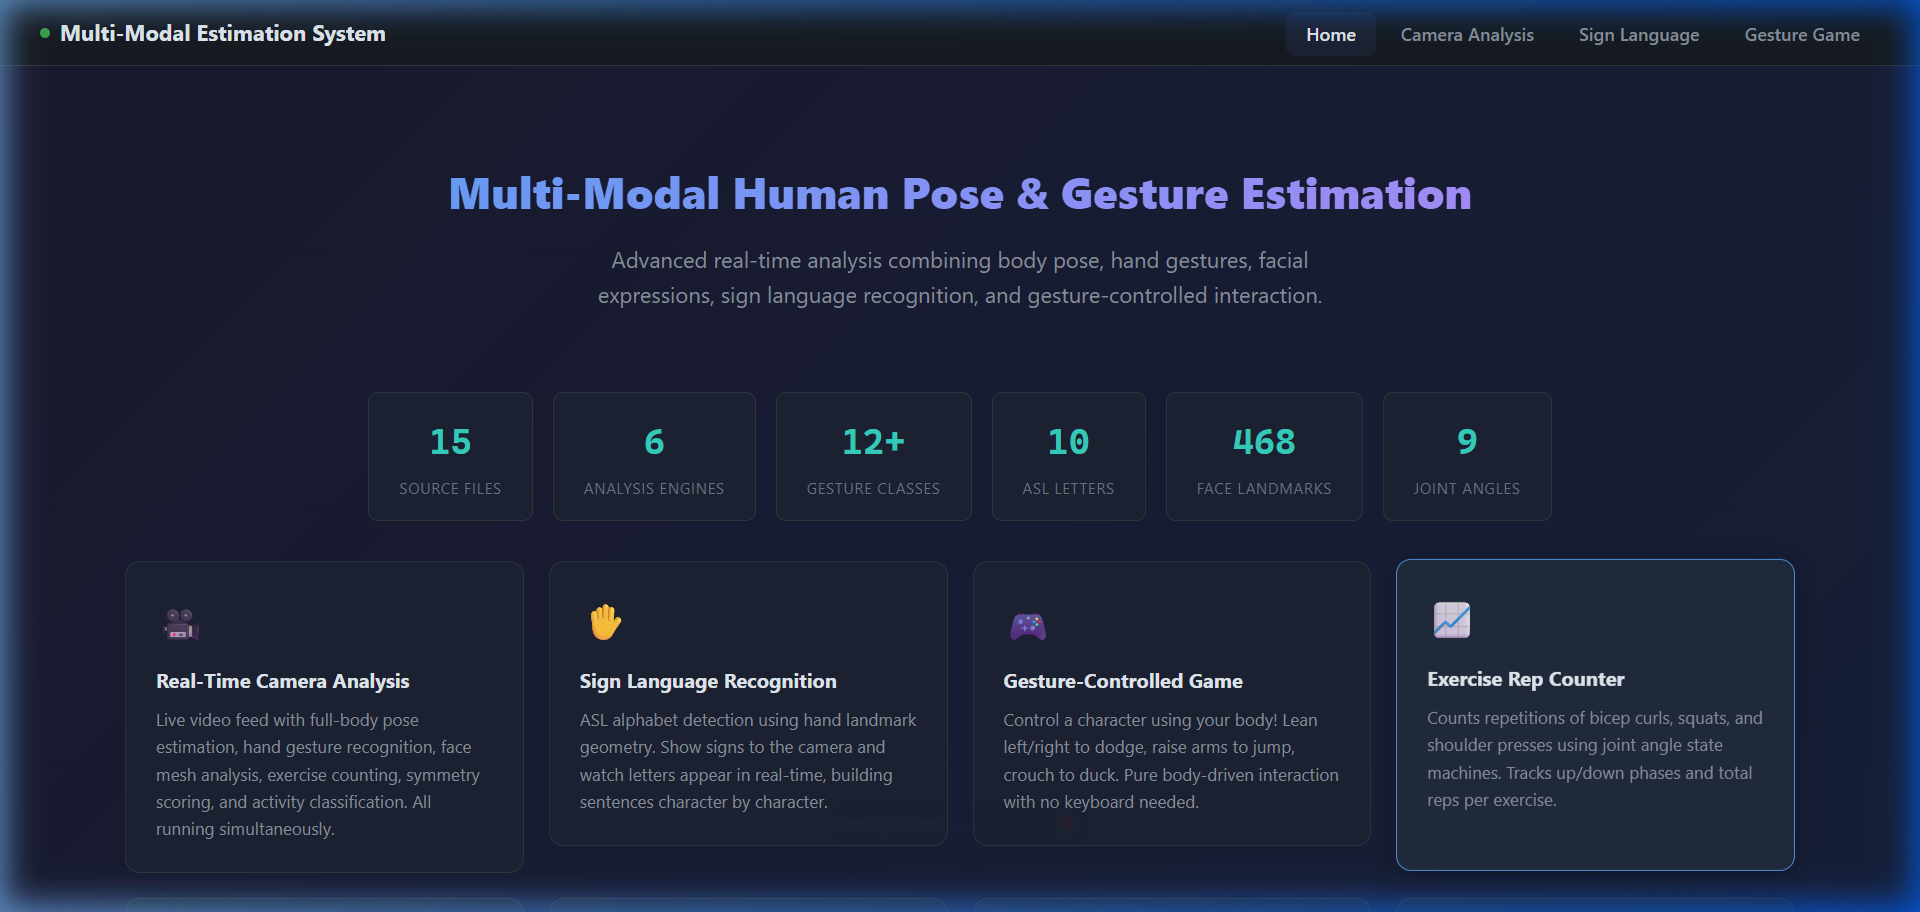
\includegraphics[width=0.95\textwidth]{../screenshots/home_page.png}
    \caption{Web Dashboard Home Page -- Feature cards and system statistics}
    \label{fig:home}
\end{figure}

\subsection{Camera Analysis Page}
Real-time video feed with module toggle controls and analytics side panels displaying pose angles, hand gestures, face metrics, activity, exercise counters, and symmetry scores.

\begin{figure}[H]
    \centering
    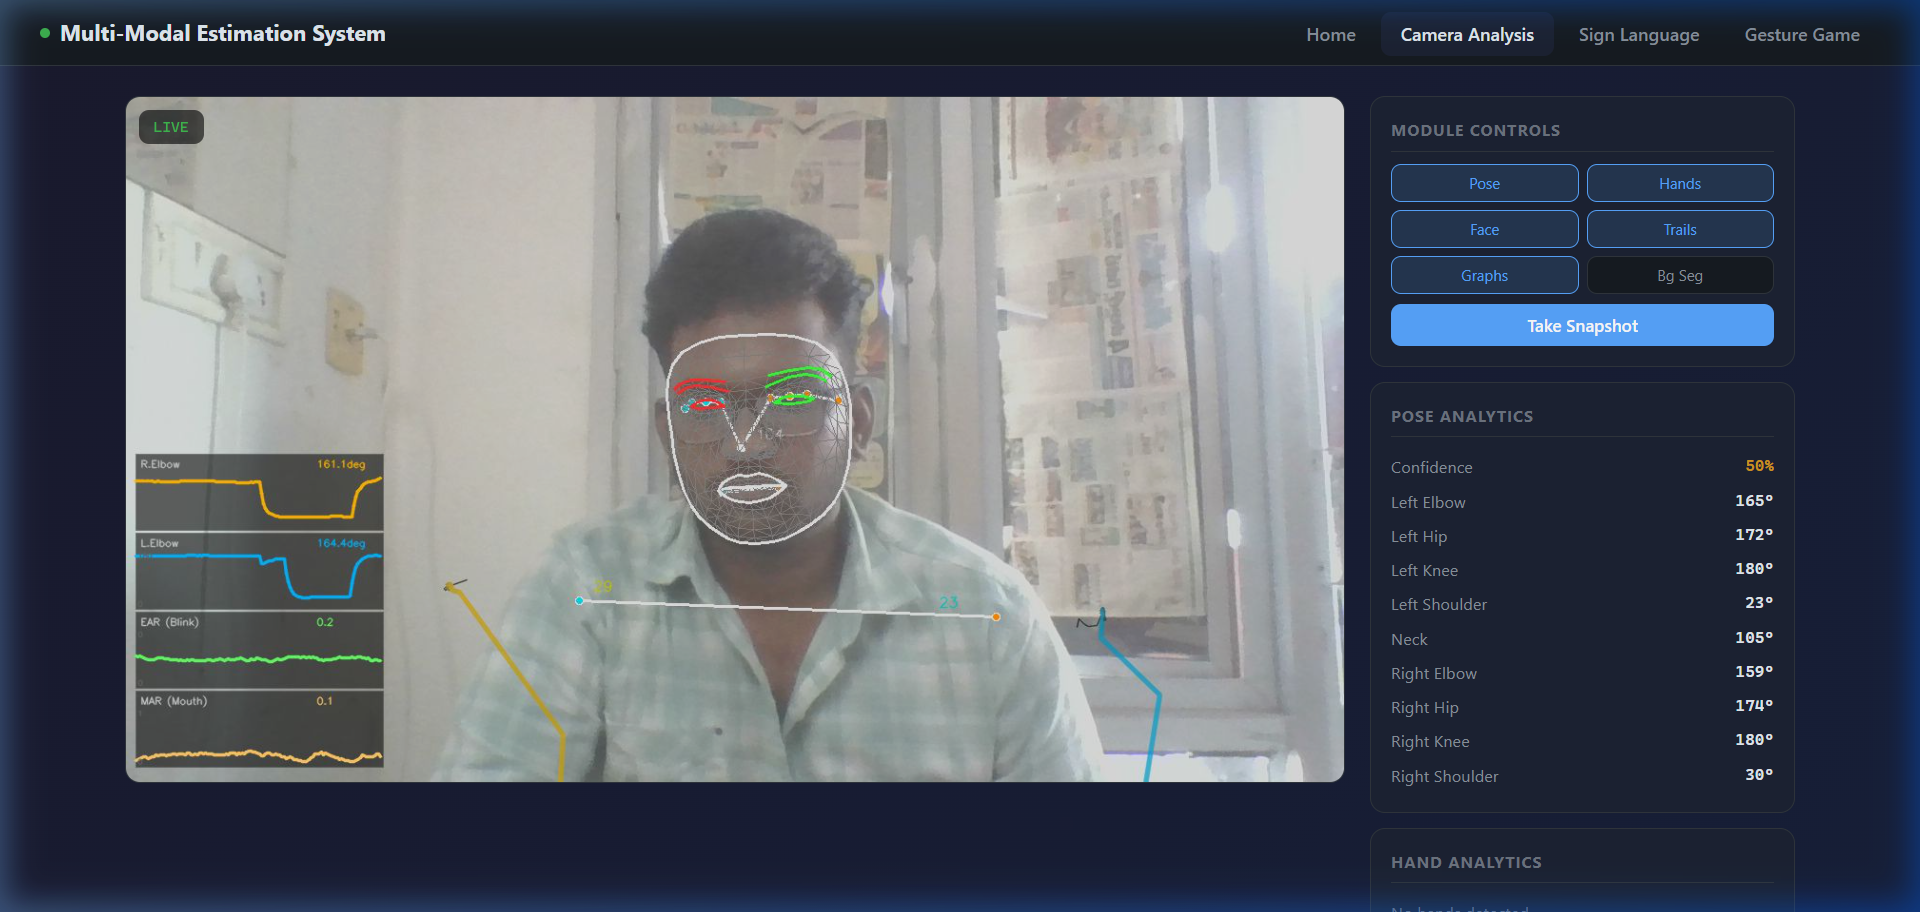
\includegraphics[width=0.95\textwidth]{../screenshots/camera_page.png}
    \caption{Camera Analysis Page -- Live video with analytics panels}
    \label{fig:camera}
\end{figure}

\subsection{Sign Language Page}
ASL alphabet detection with large detected-letter display and sentence builder. Supports Space, Backspace, and Clear controls.

\begin{figure}[H]
    \centering
    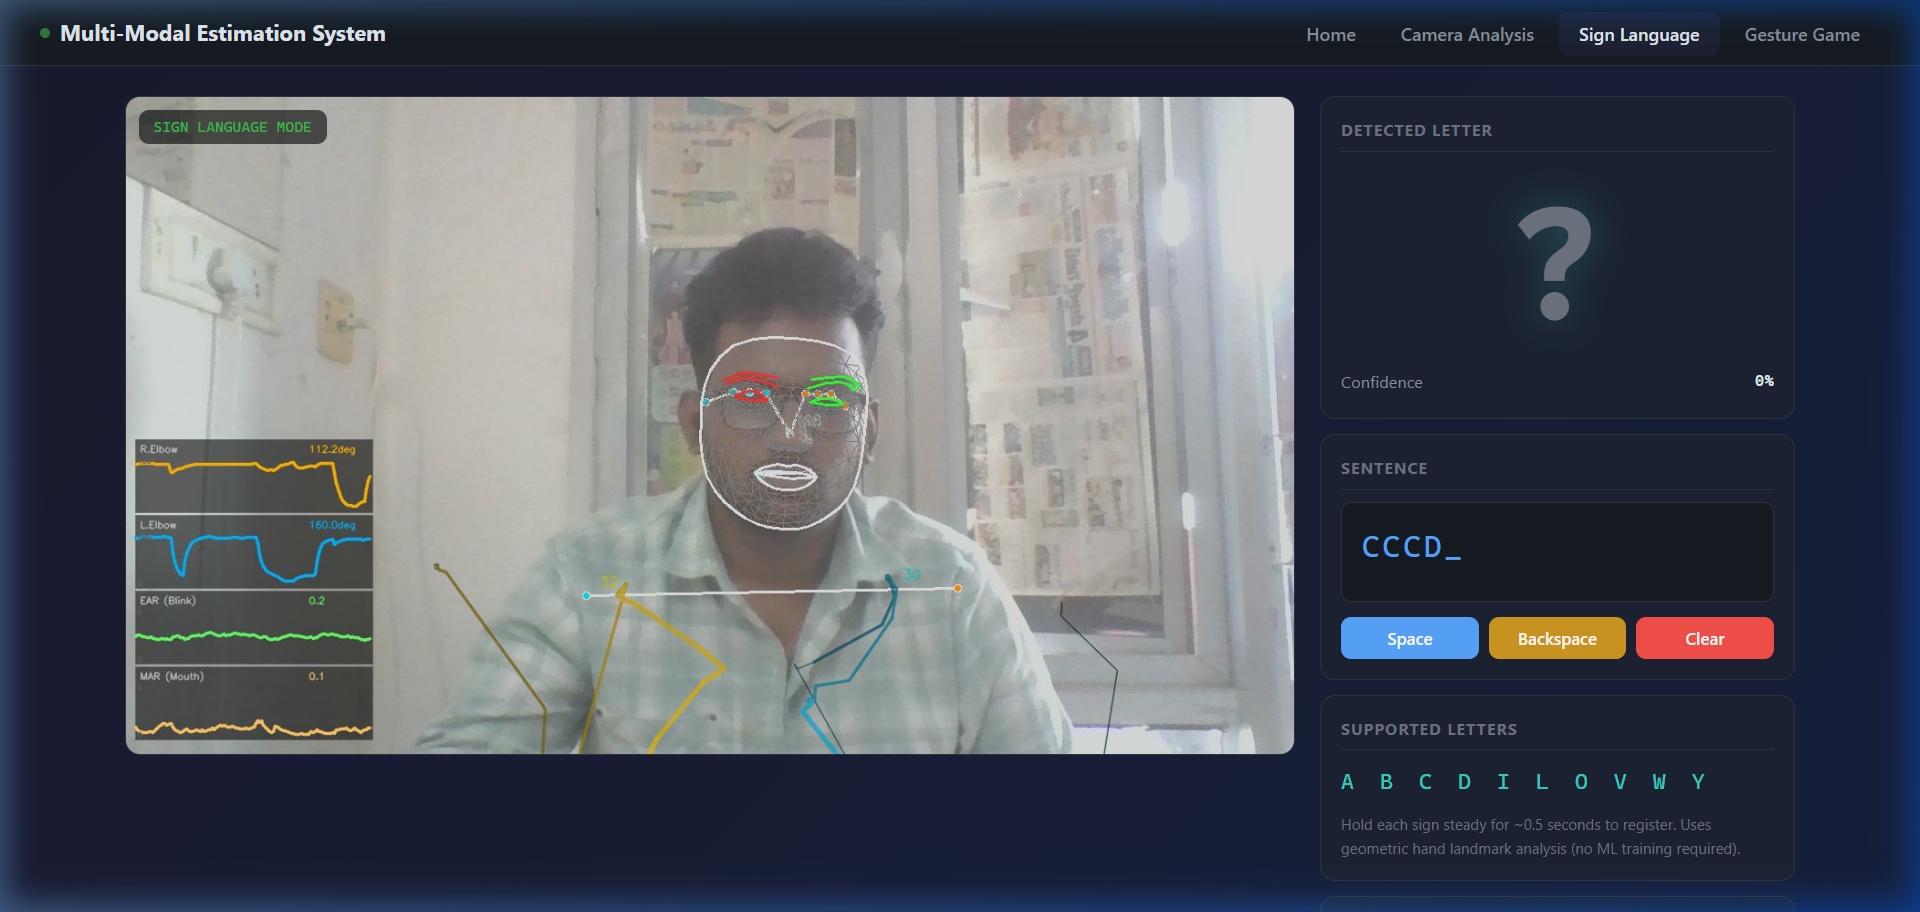
\includegraphics[width=0.95\textwidth]{../screenshots/sign_language_page.png}
    \caption{Sign Language Recognition Page -- Letter detection and sentence builder}
    \label{fig:sign}
\end{figure}

\subsection{Gesture Game Page}
Body-controlled HTML5 Canvas dodging game with camera preview showing body controls.

\begin{figure}[H]
    \centering
    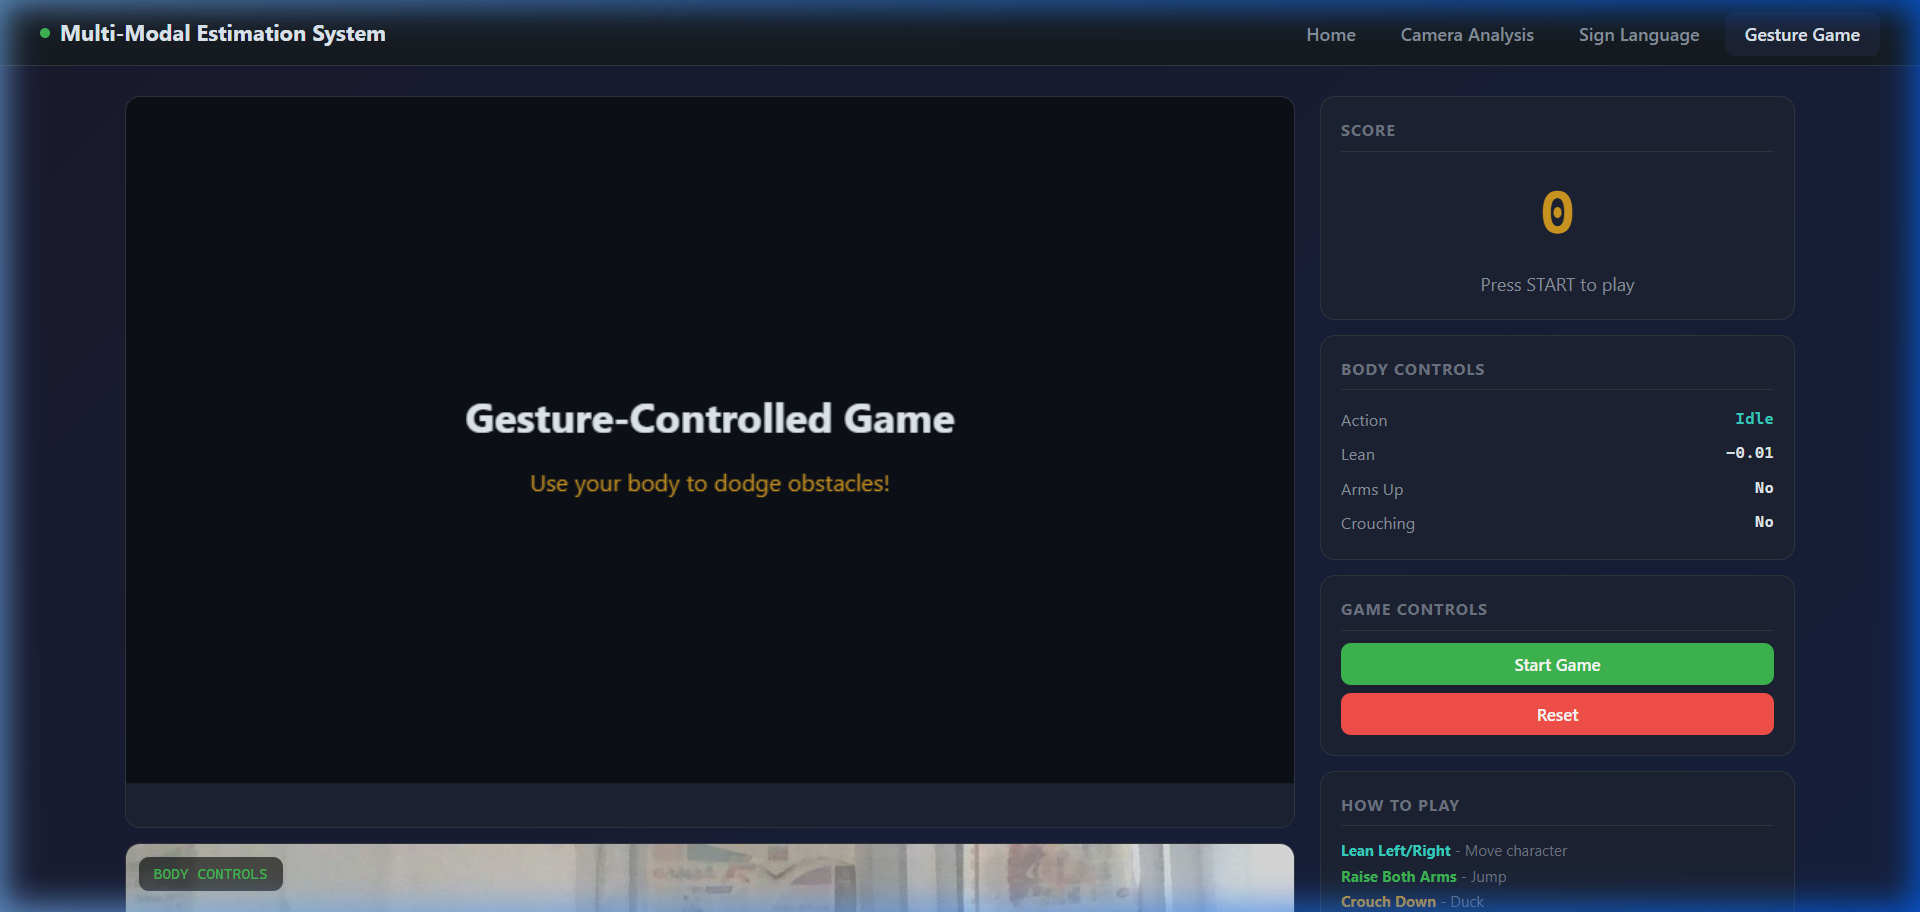
\includegraphics[width=0.95\textwidth]{../screenshots/game_page.png}
    \caption{Gesture-Controlled Game Page -- Canvas game and body control indicators}
    \label{fig:game}
\end{figure}

\section{API Endpoints}

\begin{table}[H]
\centering
\small
\begin{tabular}{|l|l|l|}
\hline
\textbf{Method} & \textbf{Endpoint} & \textbf{Description} \\
\hline
GET & \texttt{/} & Home page \\
GET & \texttt{/camera} & Camera analysis page \\
GET & \texttt{/sign-language} & Sign language page \\
GET & \texttt{/game} & Gesture game page \\
GET & \texttt{/video\_feed} & MJPEG video stream \\
GET & \texttt{/api/analytics} & JSON analytics data \\
GET & \texttt{/api/sign\_language} & JSON detected letter \\
GET & \texttt{/api/game\_state} & JSON player position \\
POST & \texttt{/api/toggle/<module>} & Toggle module on/off \\
POST & \texttt{/api/snapshot} & Take screenshot \\
\hline
\end{tabular}
\caption{Flask API Endpoint Reference}
\label{tab:api}
\end{table}

\newpage

% ================================================================
% Chapter 7: Gesture-Controlled Game
% ================================================================
\chapter{Gesture-Controlled Game}
\thispagestyle{contentpages}
\justifying

\section{Game Design}
The system includes an HTML5 Canvas-based dodging game controlled entirely by body movement -- no keyboard or mouse required.

\section{Body-to-Game Mapping}
\begin{itemize}
    \item \textbf{Move Left/Right:} Lean body (shoulder center offset from hip center)
    \item \textbf{Jump:} Raise both arms above shoulder level
    \item \textbf{Duck:} Crouch down (knees close to hips), reduces hitbox by 60\%
\end{itemize}

The player position is computed as:
\begin{equation}
    x_{\text{player}} = x_{\text{center}} + \text{lean} \times 0.4 \times W_{\text{canvas}}
\end{equation}

where $\text{lean} = \frac{x_{\text{shoulder\_center}} - x_{\text{hip\_center}}}{W_{\text{shoulder}}}$, clamped to $[-1, 1]$.

\section{Game Mechanics}
\begin{itemize}
    \item \textbf{Obstacles:} Ground-level (must dodge/jump) and elevated (must duck)
    \item \textbf{Scoring:} Score increments every 6 frames of survival
    \item \textbf{Difficulty:} Speed increases every 300 frames; spawn interval decreases
    \item \textbf{Collision:} Axis-Aligned Bounding Box (AABB) detection
    \item \textbf{Visual Effects:} Glow effects on obstacles, particle explosion on game over
\end{itemize}

\newpage

% ================================================================
% Chapter 8: Advanced Visualizations
% ================================================================
\chapter{Advanced Visualizations}
\thispagestyle{contentpages}
\justifying

\section{Motion Trajectory Trails}
The \texttt{TrailRenderer} draws fading motion trails for 4 joints:
\begin{itemize}
    \item 40-frame circular buffer per joint (L/R wrists, L/R ankles)
    \item Line segments with decreasing thickness and color intensity
    \item Alpha-blended overlay (70/30 blend ratio) for glow effect
    \item Color-coded: orange (R.Wrist), cyan (L.Wrist), red-orange (R.Ankle), blue (L.Ankle)
\end{itemize}

\section{Real-Time Scrolling Graphs}
The \texttt{GraphPanel} renders 4 live strip charts on the video frame:
\begin{itemize}
    \item \textbf{R.Elbow Angle:} $[0^{\circ}, 180^{\circ}]$, orange line
    \item \textbf{L.Elbow Angle:} $[0^{\circ}, 180^{\circ}]$, cyan line
    \item \textbf{EAR (Blink):} $[0.0, 0.5]$, green line
    \item \textbf{MAR (Mouth):} $[0.0, 1.0]$, yellow line
\end{itemize}
Each graph has a 120-frame scrolling window with semi-transparent background.

\section{Multi-Panel HUD}
The standalone OpenCV mode displays a 5-panel heads-up display:
\begin{enumerate}
    \item \textbf{Activity Panel:} Current classified posture
    \item \textbf{Pose Panel:} 9 joint angles with bar visualizations
    \item \textbf{Hand Panel:} Gesture name, finger states, openness
    \item \textbf{Exercise Panel:} Rep counts and current phase per exercise
    \item \textbf{Symmetry Panel:} Per-pair and overall symmetry scores
\end{enumerate}

\newpage

% ================================================================
% Chapter 9: Testing and Results
% ================================================================
\chapter{Testing and Results}
\thispagestyle{contentpages}
\justifying

\section{Test Methodology}
Comprehensive testing was conducted across multiple dimensions:
\begin{itemize}
    \item \textbf{Unit Testing:} Mathematical function validation
    \item \textbf{Integration Testing:} Full pipeline import and module interaction
    \item \textbf{Manual Testing:} Live webcam verification of all features
    \item \textbf{Web Testing:} Dashboard page rendering and API responses
\end{itemize}

\section{Automated Test Results}

\begin{table}[H]
\centering
\begin{tabular}{|l|l|l|}
\hline
\textbf{Test Case} & \textbf{Expected} & \textbf{Status} \\
\hline
All 20+ module imports & No errors & Pass \\
90-degree angle calculation & $90.0^{\circ}$ & Pass \\
Euclidean distance (3-4-5 triangle) & $5.0$ & Pass \\
EMA filter convergence & Approaches target & Pass \\
Exercise rep detection (bicep curl cycle) & 1 rep & Pass \\
Symmetry score (perfect match) & $100.0\%$ & Pass \\
Symmetry score (30-degree diff) & $87.5\%$ & Pass \\
Flask app imports & No errors & Pass \\
Dashboard page render (all 4 pages) & HTTP 200 & Pass \\
Analytics API response & Valid JSON & Pass \\
\hline
\end{tabular}
\caption{Automated Test Results}
\label{tab:tests}
\end{table}

\section{Performance Metrics}

\begin{table}[H]
\centering
\begin{tabular}{|l|c|}
\hline
\textbf{Metric} & \textbf{Value} \\
\hline
Frame Resolution & 1280 $\times$ 720 \\
Average FPS (all modules on) & 15--25 FPS \\
Pose Landmarks per Frame & 33 \\
Hand Landmarks per Hand & 21 (up to 2 hands) \\
Face Landmarks per Face & 468 \\
Joint Angle Computation Time & $< 1$ ms per frame \\
Activity Classification Latency & $\sim$320 ms (8 frames at 25 FPS) \\
\hline
\end{tabular}
\caption{System Performance Metrics}
\label{tab:performance}
\end{table}

\newpage

% ================================================================
% Chapter 10: Challenges and Solutions
% ================================================================
\chapter{Challenges and Solutions}
\thispagestyle{contentpages}
\justifying

\section{Technical Challenges}

\subsection{Landmark Jitter}
\textbf{Challenge:} Raw MediaPipe landmark positions fluctuate between frames, causing noisy angle readings and flickering classifications.

\textbf{Solution:} Implemented EMA filter bank (Equation~\ref{eq:ema}) with configurable smoothing factor per metric. $\alpha = 0.35$ for joint angles provides stability without excessive lag.

\subsection{Activity Classification Flickering}
\textbf{Challenge:} Frame-by-frame classification oscillates between states at posture boundaries.

\textbf{Solution:} 8-frame temporal debounce (Equation~\ref{eq:debounce}) requires consistent classification before state transition.

\subsection{Thread-Safe Video Streaming}
\textbf{Challenge:} Flask serves HTTP requests on multiple threads while the camera runs in a background thread.

\textbf{Solution:} Used \texttt{threading.Lock} for all shared state access (current frame, analytics data). MJPEG streaming via generator function with \texttt{multipart/x-mixed-replace}.

\subsection{Sign Language Ambiguity}
\textbf{Challenge:} Some ASL letters have similar hand shapes (e.g., A vs O, V vs Peace).

\textbf{Solution:} Multi-constraint matching combining finger states, inter-landmark distances, and spatial relationships. Confidence scores rank competing matches.

\section{Design Challenges}

\subsection{Modular Integration}
\textbf{Challenge:} Integrating 7 analysis engines without creating tight coupling.

\textbf{Solution:} Each engine has a standardized interface: \texttt{process\_frame(img)} returns annotated image, \texttt{get\_*\_data()} returns analytics dict. Stream manager orchestrates all engines.

\subsection{Web vs Standalone Mode}
\textbf{Challenge:} Supporting both OpenCV window and web dashboard with shared analysis code.

\textbf{Solution:} Analysis engines are mode-agnostic. \texttt{main.py} uses OpenCV display; \texttt{app.py} uses Flask MJPEG. Both instantiate the same engine classes.

\newpage

% ================================================================
% Chapter 11: Conclusion and Future Scope
% ================================================================
\chapter{Conclusion and Future Scope}
\thispagestyle{contentpages}
\justifying

\section{Project Summary}
The Multi-Modal Human Pose \& Gesture Estimation System successfully integrates seven analysis engines, a web dashboard, a sign language recognizer, and a gesture-controlled game into a cohesive real-time application. Key achievements include:

\begin{itemize}
    \item \textbf{Comprehensive Analysis:} 9 joint angles, 12+ gestures, EAR/MAR, 7 activities, 5 exercises, symmetry scoring
    \item \textbf{Sign Language:} 20 ASL letters recognized via pure geometric rules (no ML training)
    \item \textbf{Interactive Game:} Body-controlled dodging game with jump, duck, and lean
    \item \textbf{Web Dashboard:} 4-page browser interface with live video and analytics
    \item \textbf{Modular Architecture:} 25+ source files with clear separation of concerns
    \item \textbf{Dual Mode:} Standalone OpenCV (11 shortcuts) and web-based Flask interface
\end{itemize}

\section{Technical Contributions}
\begin{enumerate}
    \item \textbf{Multi-Modal Pipeline:} Simultaneous pose, hand, face processing from single webcam
    \item \textbf{20-Letter Gesture Set:} Rigorous mathematical foundation for sign detection
    \item \textbf{Body-Driven Game:} Novel mapping from pose data to interactive game controls
    \item \textbf{Premium Web UI:} Dark-themed responsive dashboard with real-time MJPEG streaming
\end{enumerate}

\section{Lessons Learned}
\begin{itemize}
    \item \textbf{Smoothing is Essential:} Raw landmark data is too noisy for direct use
    \item \textbf{Debouncing Prevents Flicker:} Temporal stability filters are critical for classification
    \item \textbf{Modularity Enables Growth:} Well-defined interfaces allow adding new engines easily
    \item \textbf{MJPEG is Pragmatic:} Simple and reliable for real-time video in web apps
\end{itemize}

\section{Future Work}
\begin{enumerate}
    \item \textbf{Deep Learning Sign Language:} LSTM/Transformer for dynamic sign sequences
    \item \textbf{Motion Prediction:} GNNs on skeleton sequences to predict future poses
    \item \textbf{Multi-Person Tracking:} Simultaneous multi-person analysis
    \item \textbf{3D Pose Reconstruction:} Depth estimation for true 3D joint positions
    \item \textbf{Cloud Deployment:} Remote access via cloud infrastructure
    \item \textbf{Mobile App:} TensorFlow Lite port for mobile platforms
\end{enumerate}

\newpage

% ================================================================
% Appendices
% ================================================================
\appendix

\chapter{Installation and Setup Guide}
\thispagestyle{contentpages}

\section{System Requirements}
\begin{itemize}
    \item \textbf{Operating System:} Windows 10/11, Linux, or macOS
    \item \textbf{Python:} 3.8 or higher
    \item \textbf{Webcam:} Any USB or built-in webcam
    \item \textbf{RAM:} 4 GB minimum (8 GB recommended)
\end{itemize}

\section{Installation Steps}
\begin{lstlisting}[language=bash, caption=Installation Commands]
# 1. Clone or navigate to the project directory
cd MM

# 2. Create virtual environment
python -m venv venv

# 3. Activate virtual environment
# Windows:
venv\Scripts\activate
# Linux/macOS:
source venv/bin/activate

# 4. Install dependencies
pip install -r requirements.txt

# 5. Run Web Dashboard
python app.py
# Open http://localhost:5000 in browser

# 6. OR Run Standalone OpenCV Mode
python main.py
\end{lstlisting}

\section{Command Reference}

\begin{table}[H]
\centering
\begin{tabular}{|l|p{8cm}|}
\hline
\textbf{Command / Key} & \textbf{Description} \\
\hline
\texttt{python app.py} & Launch web dashboard on port 5000 \\
\texttt{python main.py} & Launch standalone OpenCV mode \\
\texttt{P} & Toggle pose estimation \\
\texttt{H} & Toggle hand tracking \\
\texttt{F} & Toggle face mesh \\
\texttt{T} & Toggle motion trails \\
\texttt{G} & Toggle graphs \\
\texttt{B} & Cycle background segmentation \\
\texttt{R} & Toggle CSV recording \\
\texttt{V} & Toggle video recording \\
\texttt{S} & Take snapshot \\
\texttt{X} & Reset exercise counters \\
\texttt{Q} & Quit \\
\hline
\end{tabular}
\caption{Command and Keyboard Shortcut Reference}
\label{tab:commands}
\end{table}

\newpage

\chapter{Key Code Listings}
\thispagestyle{contentpages}

\section{EMA Filter Implementation}
\begin{lstlisting}[language=Python, caption=Exponential Moving Average Filter]
class EMAFilter:
    """Single-channel EMA smoother."""
    def __init__(self, alpha=0.35):
        self.alpha = alpha
        self._val = None

    def update(self, raw):
        if raw is None:
            return self._val
        if self._val is None:
            self._val = raw
        else:
            self._val = self.alpha * raw + (1 - self.alpha) * self._val
        return self._val
\end{lstlisting}

\section{Exercise Rep Counter State Machine}
\begin{lstlisting}[language=Python, caption=Exercise State Machine Logic]
def _update_exercise(self, exercise, angle):
    if angle is None:
        return
    if angle < exercise['thresh_down']:
        if exercise['phase'] == 'up':
            exercise['reps'] += 1
        exercise['phase'] = 'down'
    elif angle > exercise['thresh_up']:
        exercise['phase'] = 'up'
\end{lstlisting}

\section{Flask MJPEG Stream Generator}
\begin{lstlisting}[language=Python, caption=MJPEG Frame Generator for Flask]
def _mjpeg_generator():
    while True:
        frame = _stream.get_frame_jpeg()
        if frame is not None:
            yield (b'--frame\r\n'
                   b'Content-Type: image/jpeg\r\n\r\n'
                   + frame + b'\r\n')
        else:
            time.sleep(0.05)

@bp.route('/video_feed')
def video_feed():
    return Response(_mjpeg_generator(),
        mimetype='multipart/x-mixed-replace; boundary=frame')
\end{lstlisting}

% ================================================================
% Chapter 6: Premium HCI & Form-Checking Heuristics
% ================================================================
\chapter{Premium HCI \& Form-Checking Heuristics}
\thispagestyle{contentpages}
\justifying

In the final phase of development (Phase 5: Perfection Pass), the system was upgraded from a functional prototype to a premium Human-Computer Interaction (HCI) tool. This chapter details the advanced geometric heuristics implemented for physical form validation and the "Neon" visual aesthetic designed for maximum user engagement.

\section{Posture and Spine Alignment Heuristic}
To monitor user health during sitting or exercise (like planks), a spine alignment check was implemented. The system computes the midpoint of the shoulders $M_s$ and the midpoint of the hips $M_h$. The spine vector $V_{spine} = M_s - M_h$ is then analyzed for its inclination angle $\theta$:

\[ \theta = \arctan2(|dy|, |dx|) \]

where $(dx, dy)$ are the components of $V_{spine}$. In a standard vertical posture (sitting/standing), $\theta \approx 90^\circ$. If $\theta < 65^\circ$, the system flags "Slouching" and triggers a real-time toast notification on the dashboard to warn the user.

\section{Landmark-Based Squat Depth Validation}
While angle-based counters can detect repetitions, they often fail to distinguish between a "half-squat" and a full "perfect" squat. To solve this, a dual-layer validation was implemented:
\begin{enumerate}
    \item \textbf{Angle Trigger:} The knee angle must drop below $90^\circ$ to enter the "Down" phase.
    \item \textbf{Geometric Depth Check:} The $y$-coordinate of the hip landmark $(L_{24})$ must be greater than or equal to the $y$-coordinate of the knee landmark $(L_{26}) - 10$ pixels. This ensuring the hip "breaks the plane" of the knee.
\end{enumerate}
If both conditions are met, the rep is marked as "GOOD DEPTH" and counted. Otherwise, the user is prompted to "Go deeper next time".

\section{Phase 6: Advanced ASL Expansion (20 Letters)}
Building upon the initial 10-letter prototype, the system was expanded to support a near-complete static ASL alphabet (A, B, C, D, E, F, G, H, I, K, L, O, P, Q, R, S, U, V, W, Y). This required additional geometric heuristics to handle orientation and finger crossing.

\begin{enumerate}
    \item \textbf{Orientation-Awareness:} Distinguished between horizontal signs (G/H) and downward signs (P/Q) by analyzing the tip-to-MCP y-coordinate vectors.
    \item \textbf{High-Precision Fist logic:} Improved discrimination between 'A' (thumb aside), 'S' (thumb over fingers), and 'E' (thumb tucked) using specific Euclidean distance thresholds to the index knuckle.
    \item \textbf{Finger Crossing:} Letter 'R' was implemented by detecting a crossing event where the Euclidean distance between index and middle tips is less than 15\% of the wrist-middle distance while both are extended.
\end{enumerate}

This expansion brings the total supported vocabulary to 20 letters, making the system viable for spelling complex English words in real-time.

\section{Premium Visual Aesthetics: Neon Skeleton Drawing}
To create a "WOW" factor for presentation, the standard MediaPipe skeleton dots were replaced with a custom \textbf{Neon-Style HUD}. This uses a multi-pass drawing algorithm:
\begin{itemize}
    \item \textbf{Pass 1: Glow Generation.} A thick, semi-transparent line is drawn with a Gaussian blur-like effect using \textbf{cyan} for normal states and \textbf{orange} for alert states (e.g., Slouching).
    \item \textbf{Pass 2: Bone Core.} A thin, bright white line is drawn over the glow to simulate a light-tube effect.
    \item \textbf{Pass 3: Joint Highlights.} Circular markers are added at major kinematic joints with a matching glow.
\end{itemize}
This visual style significantly improves the professional feel of the dashboard compared to standard skeletal overlays.

% ================================================================
% References
% ================================================================
\newpage
\addcontentsline{toc}{chapter}{References}
\bibliographystyle{plain}
\bibliography{references}

\end{document}
